%%%%%%%%%%%%%%%%%%%%%%%%%%%%%%%%%%%%%%%%%%%%%%%%%%%%%%%%%%%%%%%%%%%%%%%%%%%%%%%
% June 2021, R. Schoetter, created based on GMD article by Auguste et al. (2020).
%%%%%%%%%%%%%%%%%%%%%%%%%%%%%%%%%%%%%%%%%%%%%%%%%%%%%%%%%%%%%%%%%%%%%%%%%%%%%%%
%
\chapter{Immersed Boundaries}
\minitoc
%
\section{Introduction}
%
This chapter has been adapted from Auguste et al. (2019) and presents the implementation 
of an Immersed Boundary Method (IBM) in Meso-NH to represent obstacles for simulations 
using a cartesian grid and flat terrain. Only the fundamental equations related to the 
IBM are given here, examples of IBM validation and application are given in 
Auguste et al. (2019). \\
%
Numerical solvers in Meso-NH enforce conservation on structured grids and hence cannot 
handle body fitted grids with steep topological gradients. The main idea behind the IBM 
is the detection of an interface separating a fluid region, where conservations laws 
are valid, from a solid region corresponding to the obstacle volume, by using different 
techniques (e.g. markers, LevelSet functions, local volume fraction, etc). 
Two main classes of IBM exist, which are based on the continuous and discrete forcing 
approaches, respectively. The continuous forcing approach was developed by Peskin (1972) 
for biomechanics applications and consists in the addition of a continuous artificial 
force in the momentum conservation equation that mimics the effect of the obstacles and 
drives the flow to relax to a no-slip condition at the wall of the obstacle. This approach 
and its variant developed by Goldstein et al. (1993) for a rigid interface can suffer 
from the lack of stiffness since the fluid-solid interface is generally spread over 
few cells, and the time step restriction. For the discrete approach, 
the boundary conditions are specified at the immersed interface. To simulate flows 
around non moving and rigid bodies, two subclasses of discrete approaches can be 
defined as in Mittal and Iaccarino (2005): direct or indirect approaches, depending 
on the forcing location (Pierson, 2015). Many types of discrete forcing exist, e.g. 
direct forcing in the fluid region near the interface as in Mohd-Yusof (1997), the 
immersed interface method (Leveque and Li, 1994), or the Cartesian grid method (Clarke et al., 1986). 
Depending on how to resolve the partial differential equations, Cartesian grid methods 
(Ye et al., 1999) are written for finite-volume discretizations (Cut-Cell Technique, CCT) 
and for finite-difference discretizations (Ghost-Cell Technique, GCT) as in 
Tseng and Ferziger (2003). The CCT reshapes the cell cut by the interface to preserve mass, 
momentum and energy. Using GCT, the local spatial reconstruction is done inside the 
solid region. The latter technique has been successfully implemented by Lundquist et al. (2010, 2012)
in the Weather Research and Forecasting (WRF) model. \\
%
The IBM implemented in Meso-NH is based on the discrete forcing approach. 
The fluid-solid interface is modelled by means of a LevelSet function 
(Sussman et al., 1994). The motivation behind this choice is that rigid 
and non-moving bodies in a turbulent flow shall be represented, and with 
sufficiently fine resolution to avoid the large dissipation inherent to 
the presumed spread interface. The GCT does not introduce source terms in 
the conservation equations modelling the fluid region so that boundary conditions 
are imposed at the interface and/or in the solid region. The only corrections 
to the physical model in the fluid region come from subgrid turbulent parameterizations. 
The idea is that in mesoscale atmospheric modelling applications, the IBM is 
used to resolve large obstacles such as buildings or mountains, whereas a 
subgrid drag model is used to handle unresolved obstacles 
such as vegetation (Aumond et al., 2013).
%
\section{Representation of obstacles via a LevelSet function}
\label{S_IBM}
%
The numerical domain is divided in two regions: a fluid region where the equations of continuum 
mechanics hold, and a solid region embedding the obstacle where they do not. 
After comparing two methods to represent the obstacles (Fig.~\ref{mesh_nodeX}-a), one
based on a local presence function, and one based on the LevelSet Function (LSF; Sussman et al., 1994; 
Kempe and Fröhlich, 2012), the LSF is chosen since it is able to 
capture the interface between the fluid and solid regions more accurately : 
The $\mid \phi \mid$ distance informs about the minimal distance to the 
fluid-solid interface and the $\phi$-sign about the region nature: sgn$(\phi)>0$ 
for the solid one; otherwise sgn$(\phi) < 0$. The vector ${\bf n}$ normal to 
the interface and its local curvature $\sigma$ are defined such as 
${\bf n} = \frac{\bf \nabla \phi}{\bf |\nabla \phi|}$ and 
$\sigma = -\nabla . {\bf n}$. Fig.~\ref{mesh_nodeX}-a illustrates the 
continuous variation of LSF for an arbitrary bell shape interface. 
The LSF is estimated at the seven available point types per grid cell to limit 
the discretization errors (Fig.~\ref{mesh_nodeX}-b): at the mass point $P$ 
where prognostic scalar variables are localized, at the three velocity 
nodes $U/V/W$, and the A/B/C vorticity nodes employed by turbulent variables. 
The points of the solid region acts as external points of the computational grid.
%
\begin{figure}[!ht]
\begin{center}
	 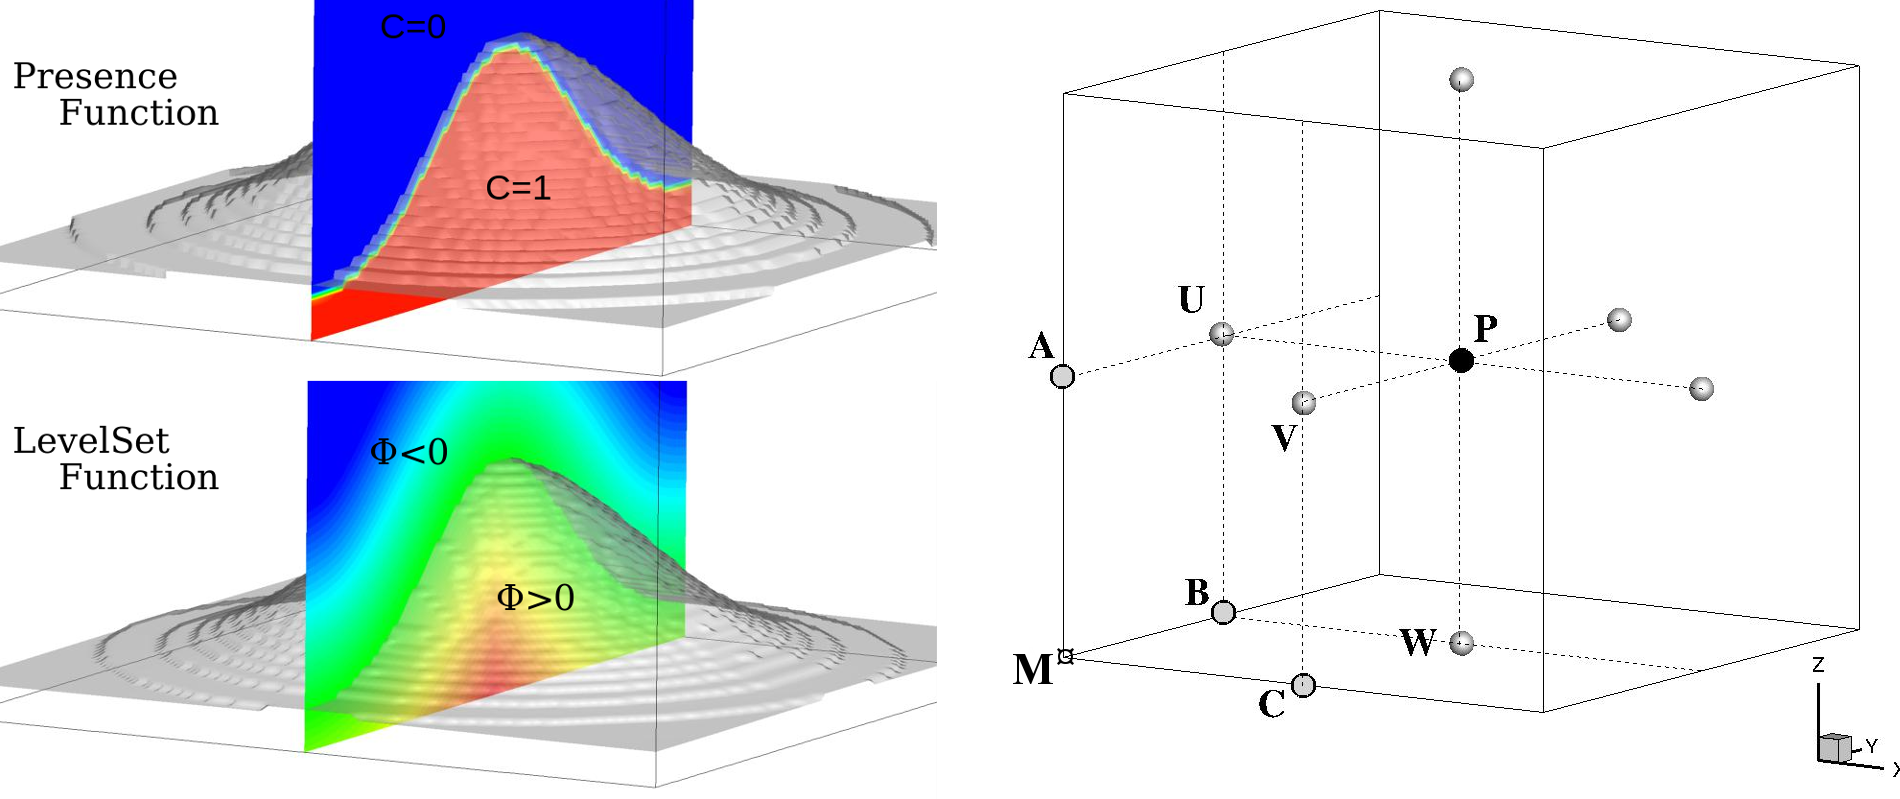
\includegraphics[width=16.cm]{\EPSDIR/fig10_1.png} \\
			\vspace{-1mm}	 	(a) \hspace{5.6cm} (b) 
	\small \caption {{\it (a) Illustration of two ways to model a fluid-solid interface: the color code indicates the isocontours of the presence function $C$ and the LevelSet function $\phi$; (b) Definition of the point types per grid cell: M the geometric/mesh point, P the mass point, U/V/W the velocity nodes and A/B/C the vorticity nodes.}}
\label{mesh_nodeX} 
\end{center}
\end{figure}
%
\section{Modification of the equations using a Ghost Cut-Cell Technique} 
\label{S_GCT}
%
Let $\psi^n$ be a prognostic variable of Meso-NH at the time $n\Delta t$ ($\Delta t$, the time step). The tendencies of the prognostic variables $\overline{\psi}=[\overline{\bf{u}},\overline{\theta},\overline{s},(e)]$ can not be deduced from the conservation laws in the solid region. Expecting a correction due to IBM where $\phi \ge 0$, a general formulation of the tendencies is written as:

\vspace{-0.25cm}
\begin{equation}
\frac{\partial }{\partial t} = \frac{\partial }{\partial t}\bigg|_{csl} + \frac{\partial }{\partial t}\bigg|_{ibm}
\label{ibmlaw}
\end{equation}
\vspace{-0.25cm}

The RHS first term of Equation~\eqref{ibmlaw} is given by the conservation laws. The $\frac{\partial}{\partial t}\big|_{ibm}$ tendency is the correction due to the GCT in the solid region and near the immersed interface satisfying the $\overline{\psi}$ desired boundary conditions at $\phi=0$:

\vspace{-0.25cm}
\begin{equation}
\frac{\partial \overline{\psi}}{\partial t}\bigg|_{ibm}=-\frac{\partial \overline{\psi}}{\partial t}\bigg|_{csl}+\frac{\overline{\psi}^{n+1}-\overline{\psi}^{n}}{\Delta t} \\
\end{equation}
\vspace{-0.25cm} 

\begin{figure}[!ht]
\begin{center}
   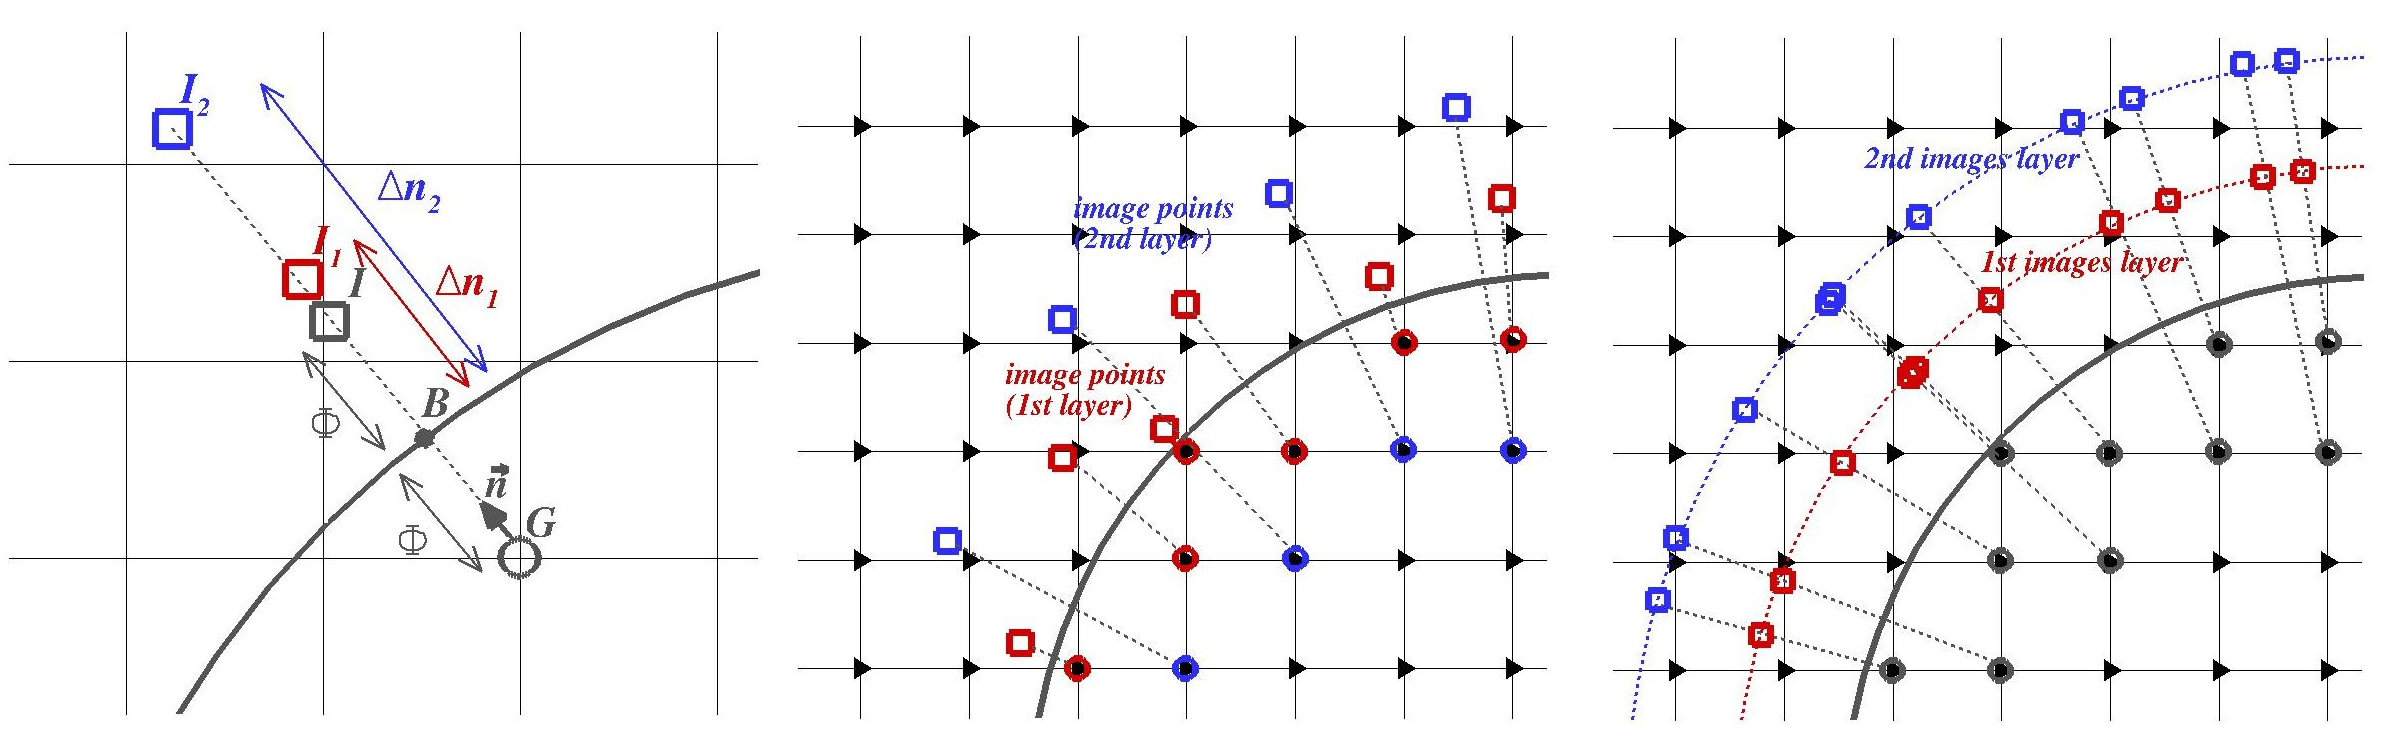
\includegraphics[width=16.cm]{\EPSDIR/fig10_2.png}	\\
		\vspace{-1mm} 	(a) \hspace{5.2cm} (b) \hspace{5.3cm} (c)
	\small \caption {{\it  (a) Node definitions acting in the Ghost-Cell Technique : the ghost ($G$), interface ($B$), normal vector (${\bf n}$), mirror ($I$) and images ($I_1,I_2$). (b resp. c) Illustration of the classical (resp. new) GCT using the mirror (resp. images). Triangles correspond to one of the node types (see Fig.~\ref{mesh_nodeX}-b).}}
	\label{ghost_image34}
\end{center}
\end{figure}

The forced points are called ghost points and merely renamed ghosts. To estimate the variable $\overline{\psi}$ and for each ghost, the physical information is extracted near the interface and from the fluid region. The extension (grid stencil) of the forcing zone depends on the spatial accuracy of the numerical scheme. For example, Figure~\ref{ghost_image34}b-c show the case of a two-layers stencil in a two-dimensional grid. The characterization of the layer is done by a conditional loop applied direction by direction on the LSF. For a 2D case, the sign of $\phi(i,j).\phi(i,[j-k_l:j+k_l])$ and $\phi(i,j).\phi([i-k_l:i+k_l],j)$ is estimated. The integer value $k_l$ determines the cells truncated by the interface: $k_l=1$ (resp. $k_l=2$) defines the first (resp. second) layer. The calculation of these ghost layers has a computational overhead due to data exchange among processors in parallel simulations. The stencil of the numerical schemes modelling the interface defines the $k_l$ value. In order to limit this overhead, a low-order version of centered explicit-in-time schemes is employed when $\phi > -\Delta$. The CPU cost of the 'hybrid' advection scheme is largely compensated by the decrease of the ghosts number and parallel exchanges.

In the classical GCT (Tseng and Ferziger, 2003), the fluid information is obtained at a mirror point (noted $I$, merely renamed mirror) found in the normal direction to the interface in such a way that the interface node $B$ is equidistant to $I$ and $G$. Figure~\ref{ghost_image34}-a shows the characterization of one ghost $G$ (of LSF value $\phi_G$), its associated mirror $I$ (of LSF value $\phi_I$) and the interface node $B$ (${\bf GI}=2\phi_G {\bf n}$). Figure~\ref{ghost_image34}-b illustrates several ghosts and mirrors. The $| {\bf IB} |$ distance depends on the forcing stencil and a problematic case regularly met in the mirror interpolation is the vicinity of ghosts with the interface ($\phi_G=-\phi_I << \Delta$, with $\Delta$ the space step) leading to a not well-posed condition. \\

{\bf The new GCT}. To overcome this problem, we define image points (noted $I_1$ and $I_2$ in Fig.~\ref{ghost_image34}-a, merely renamed images) having a distance to the interface that depends only on the grid spacing: ${\bf GI_l}=l\Delta + \phi_G {\bf n}$ with $l=(1;2)$. Figure~\ref{ghost_image34}-a shows the images for one ghost. The new approach enforces a large enough value of the $| {\bf I_lB} |$ distance. Figure~\ref{ghost_image34}-b (resp. c) illustrates the classical (resp. new) GCT for several ghosts. Figure~\ref{ghost_image34}-b shows some mirror points associated with ghosts of the first layer in the vicinity of the interface. Figure~\ref{ghost_image34}-c shows that the new approach ensures that the image points are always located in the fluid region, irrespective of the ghost location. The definition of several images per ghost allows to build a profile of the $\overline{\psi}$ fluid information normal to the interface. $\overline{\psi}(I)$ is therefore recovered by a quadratic reconstruction $f$ using the $(B,I_1,I_2)$ points. Two distinct calculations of $f(\overline{\psi}(B),\overline{\psi}(I_1),\overline{\psi}(I_2))$ noted $PLI^{a}$ and $PLI^{b}$ are tested to build the Lagrange interpolation:

\vspace{-0.25cm}
\begin{equation}
	PLI^{a}(I)=[2L^{a}_{G}(I)\overline{\psi}(B)+L^{a}_{I_1}(I)\overline{\psi}(I_1)+L^{a}_{I_2}(I)\overline{\psi}(I_2)][1+L^{a}_{G}(I)]^{-1}
\end{equation} 
\vspace{-0.25cm}	
\vspace{-0.25cm}
\begin{equation}	
	PLI^{b}(I)=L^{b}_{B}(I)\overline{\psi}(B)+L^{b}_{I_1}(I)\overline{\psi}(I_1)+L^{b}_{I_2}(I)\overline{\psi}(I_2)
\end{equation}
\vspace{-0.25cm}

where $L^{a}(I)$ and $L^{b}(I)$ are the Lagrange polynomials:

\vspace{-0.25cm}
\begin{equation}
	L^{a}_{I_1}(I)=\left( \frac{2\Delta -\phi}{\Delta }     \right) \left( \frac{2\phi}{\Delta +\phi}          \right)
\end{equation} 
\begin{equation}
	L^{a}_{I_2}(I)=\left( \frac{\phi-\Delta }{\Delta }      \right) \left( \frac{2\phi}{2\Delta +\phi}         \right)
\end{equation} 
\begin{equation}
	L^{a}_{G}(I)  =\left( \frac{\phi-\Delta }{\phi+\Delta } \right) \left( \frac{\phi-2\Delta }{\phi+2\Delta } \right)
\end{equation} 
\begin{equation}	
	L^{b}_{I_1}(I)=\left( \frac{2\Delta -\phi}{\Delta } \right) \left( \frac{\phi}{\Delta}            \right)
\end{equation} 
\begin{equation}
	L^{b}_{I_2}(I)=\left( \frac{\phi-\Delta }{\Delta }  \right) \left( \frac{\phi}{2\Delta}           \right)
\end{equation} 
\begin{equation}		
	L^{b}_{B}(I)  =\left( \frac{\phi}{\Delta}           \right) \left( \frac{\phi-2\Delta }{2\Delta } \right)  
\end{equation} 
\vspace{-0.25cm}

\begin{figure}[!ht]
	\begin{center}
		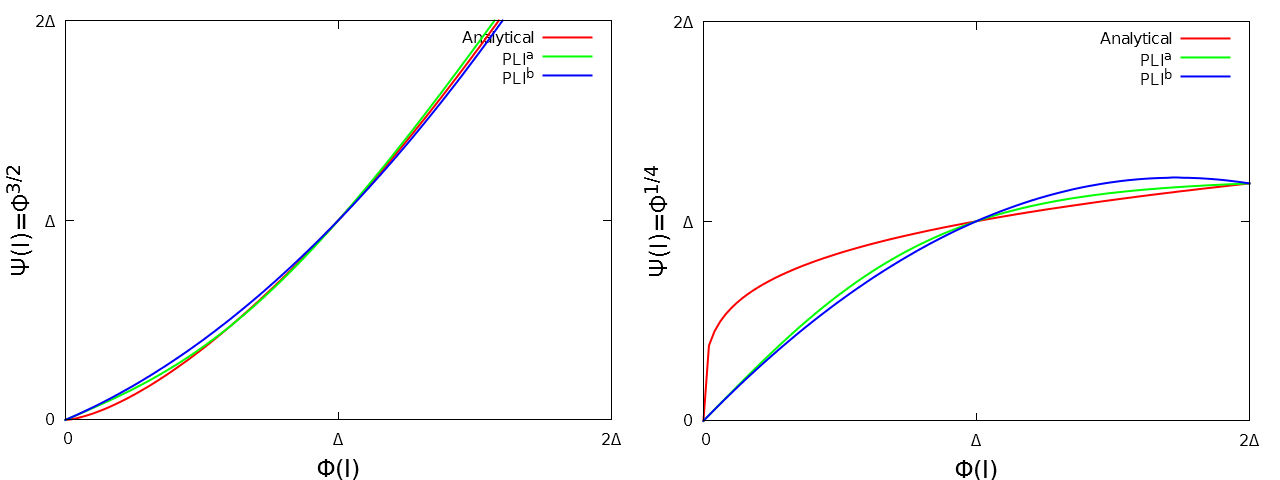
\includegraphics[width=16cm]{\EPSDIR/fig10_3.png} \\
		\vspace{-1mm} 	(a) \hspace{7cm} (b) 
		\small \caption {{\it Quadratic interpolations of two analytical profiles $\overline{\psi}=\phi^n$ (red lines) using two image points at $\phi=-[1;2]\Delta$ and the interface node. Green (resp. blue) color corresponds to $L^{a}$ (resp. $L^{b}$) polynomial results.}}
		\label{A_lag1D}	
	\end{center}
\end{figure}

The accuracy of an interpolation depends on the $\overline{\psi}$-profile. For example, a logarithmic evolution of the tangent velocity is expected in LES. Otherwise when the viscous layer is modelled, a linear evolution is expected. To compare the ability of each quadratic interpolation to approach a wide variety of profiles, the recover of power laws such as $\psi=\phi^{3/2}$ (Figure~\ref{A_lag1D}-a) and $\psi=\phi^{1/4}$ (Fig.~\ref{A_lag1D}-b) is studied. As it illustrates, $PLI^{a}$ fits better the two analytical solutions and is therefore adopted. The GCT implementation is divided in four main steps: the fluid information recovery, the interface basis change, the interface condition and the ghost value.\\

{\bf The fluid information recovery}. The values of $\overline{\psi}_{I_l}$ for the images located in a pure fluid cell (all corner nodes are in the fluid region) is recovered by a trilinear interpolation based on Lagrange Polynomials (LP):

\vspace{-0.25cm}
\begin{equation}
	L^{LP}_i(x_l)=\overset{N}{\underset{p=1,p \neq i}{\prod}}\frac{x_l-x_p}{x_i-x_p} \hspace{0.25cm} ; \hspace{0.25cm}
	L^{LP}_j(y_l)=\overset{N}{\underset{p=1,p \neq j}{\prod}}\frac{y_l-y_p}{y_j-y_p} \hspace{0.25cm} ; \hspace{0.25cm}
	L^{LP}_k(z_l)=\overset{N}{\underset{p=1,p \neq k}{\prod}}\frac{z_l-z_p}{z_k-z_p} \\
\end{equation}	
\vspace{-0.25cm}
\vspace{-0.25cm}
\begin{equation}
	\overline{\psi}(x_l,y_l,z_l)= \overset{N}{\underset{i=1}{\sum}} \overset{N}{\underset{j=1}{\sum}}  
	                   \overset{N}{\underset{k=1}{\sum}}L^{LP}_i(x_l)L^{LP}_j(y_l)L^{LP}_k(z_l).\overline{\psi}(x_i,y_j,z_k) 
\end{equation}
\vspace{-0.25cm}

For truncated cells with at least one corner node in the solid region, $\overline{\psi}_{I_l}$ is recovered using an inverse Distance Weighting (DW) interpolation:

\vspace{-0.25cm}
\begin{equation}
	\overline{\psi}(x_l)=\frac{\overset{N}{\underset{i=1}{\sum}}L^{DW}_i(x_l).\overline{\psi}(x_i)}{\overset{N}{\underset{i=1}{\sum}}L^{DW}_i(x_l)} \hspace{0.25cm} ; \hspace{0.25cm}
	\mid {\bf x_l}-{\bf x_i} \mid=\sqrt{(x_l-x_i)^2+(y_l-y_i)^2+(z_l-z_i)^2}
	\label{E_ID}
\end{equation}
\vspace{-0.25cm}

where $L^{DW}_i(x)=\mid x_l-x_i \mid^{-\alpha}$ ($\alpha=1$). This formulation diverges when $x_i \rightarrow x_l$ and it is commonly adopted to impose $\overline{\psi}(x_l)=\overline{\psi}(x_i)$ when $\exists(x_i-x_l) \leq \epsilon$ ($\epsilon$ is an arbitrary parameter depending on the mesh discretization, $\epsilon<<\Delta$). The 3D extension is direct with $\mid {\bf x_l}-{\bf x_i} \mid=\sqrt{(x_l-x_i)^2+(y_l-y_i)^2+(z_l-z_i)^2}$. This interpolation method has been chosen after comparison with Barycentric Lagrange and Modified Distance Weighting interpolations (Franke, 1982) and tests on the $\alpha$ coefficient. As the boundary condition is expressed in the interface frame and the grid is staggered, the non-collocation of the $\overline{\bf u}$ components implies firstly to interpolate three different classes of cells (with $U/V/W$ corners, Fig.~\ref{mesh_nodeX}-b) for each $U/V/W$ ghosts, secondly to build the change of frame matrix for which the proposed GCT presents an interest during the characterization of the direction tangent to the interface.\\

{\bf The interface basis change}. The velocity vector ${\bf \overline{u}}$ defined in the Cartesian mesh basis at the images $I_l$ ($\Delta n_1=\Delta$ and $\Delta n_2=2\Delta$ in Fig.~\ref{ghost_image34}-a) is projected in the basis of the interface $({\bf n}(B),{\bf t}(B),{\bf c}(B))$ in which the boundary conditions on each vector component are imposed. The normal direction to the obstacle is defined by Computing the LSF gradient. Otherwise, (${\bf t},{\bf c}$) are two arbitrary tangent directions. The tangent direction ${\bf t}$ is considered as the predominant tangent direction of the flow along the fluid-solid interface depending on the image values and defining the velocity vector such as ${\bf \overline{u}}(I_l)=\overline{u}_n(I_l){\bf n}+\overline{u}_t(I_l){\bf t}(I_l)$. The cotangent direction is defined such as:

\vspace{-0.25cm}
\begin{equation}
	{\bf c}(I_l) = \frac{{\bf n}\otimes {\bf \overline{u}}(I_l)}{\mid\mid{\bf n}\otimes{\bf \overline{u}}(I_l)\mid\mid} \hspace{0.25cm} ; \hspace{0.25cm}
	{\bf t}(I_l) = {\bf c}(I_l)\otimes{\bf n}
\end{equation}
\vspace{-0.25cm}

The $({\bf n},{\bf t},{\bf c})$ basis at the interface is defined by considering or not the rotation of the tangent velocity with the distance to the interface:

\vspace{-0.25cm}
\begin{equation}
	{\bf t}(B) = {\bf t}(I_1)  \hspace{0.1cm} \textnormal{if no rotation} \hspace{0.35cm} ; \hspace{0.35cm} {\bf e_t}(B)  =2{\bf e_t}(I_1)-{\bf e_t}(I_2)  \hspace{0.1cm} \textnormal{if linear evolution} 
\end{equation}
\vspace{-0.25cm}

Finally, the third component is ${\bf c}(B) = {\bf n}\otimes{\bf e_t}(B)$ and (inverse) projection is known.\\	

{\bf The interface condition}. Let $\overline{\psi}_B$ and $\Delta\frac{\partial \overline{\psi}}{\partial n}{\big|}_B$ the Dirichlet and Neumann conditions on $\overline{\psi}$ at boundary $B$. The general formulation of the boundary condition $\overline{\psi}(\phi=0)$ is written as a Robin condition: $\overline{\psi}(\phi=0)=k_{r}\overline{\psi}_B+(1-k_{r}).(\overline{\psi}(\phi=-l\Delta)-l\Delta\frac{\partial \overline{\psi}}{\partial n}{\big|}_B$). The switch between the Dirichlet condition and the Neumann condition is done through the coefficient $k_{r} \in [0:1]$. A Dirichlet condition, $(k_{r};\overline{\psi}_B)=(1;0)$ is imposed on the $\overline{\bf{u}}.{\bf n}$ velocity component normal to the interface arising from the impermeability hypothesis, and on the $\overline{\bf{u}}.{\bf t}$ component tangent to the interface for a no-slip hypothesis. A Neumann condition ($(k_{r};\frac{\partial \overline{\psi}}{\partial n}{\big|}_B)=(0;0)$) is imposed for potential temperature, passive scalars, and subgrid kinetic energy to represent a no surface flux boundary condition, and to represent a free-slip case for $\overline{\bf{u}}.{\bf t}$. The $\frac{l\phi}{2}$-approximation in the location of the derivative term and the Neumann condition depending on the chosen image (in practice the selected image $I_l$ is the closest one to the interface).

An interface condition depending on the characteristics of the surrounding fluid such as $\overline{\psi}(\phi=0)=F(\overline{\psi}_{I_l};\frac{\partial \overline{\psi}}{\partial n}{\big|}_{I_l})$ is a wall model. Using two (resp. three) images, simple wall models such as the constant (resp. linear) extrapolation of the $\overline{\psi}$ gradient is reached by the $\frac{\partial^2 \overline{\psi}}{\partial n^2}{\big|}_{I_l}=0$ (resp. $\frac{\partial^3 \overline{\psi}}{\partial n^3}{\big|}_{I_l}=0$) computation. The consistency between the tangent component to the interface of the resolved wind and the subgrid turbulence is the subject of Section~\ref{S_WAL}.\\

\begin{figure}[!ht]
\begin{center}
	 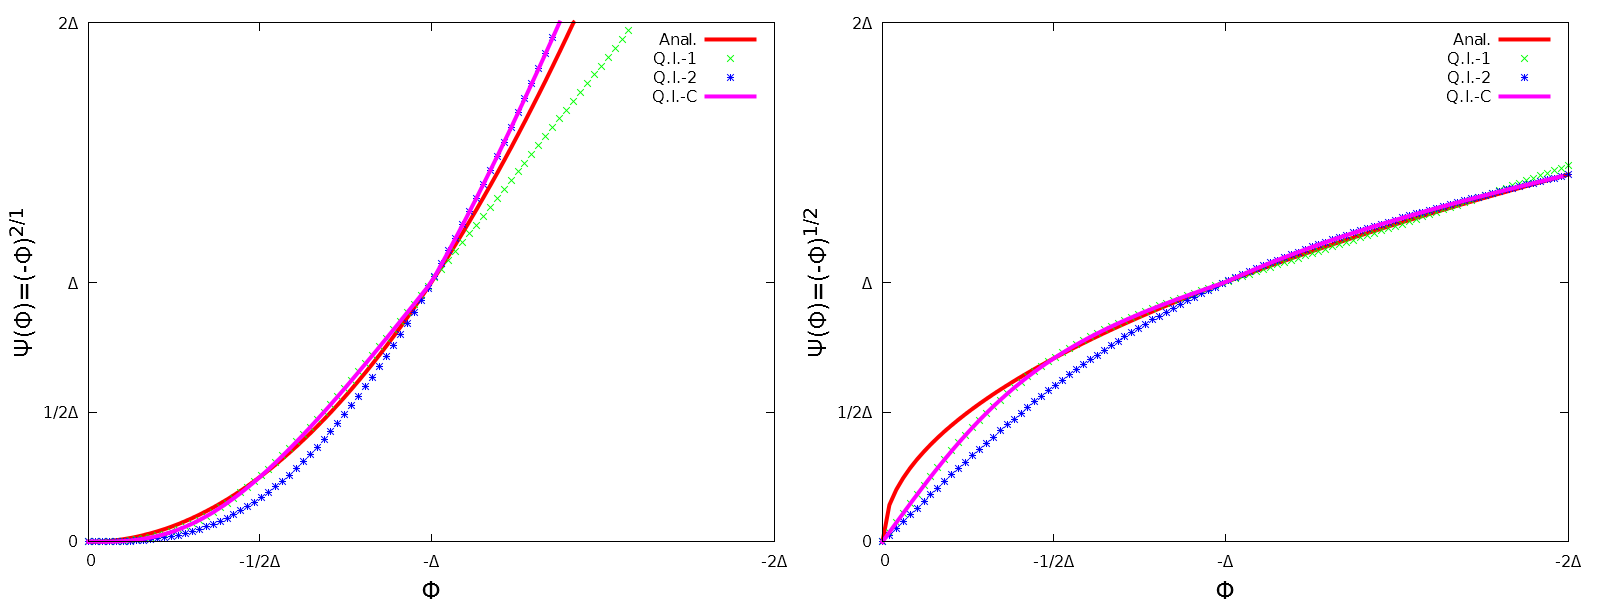
\includegraphics[width=16cm]{\EPSDIR/fig10_4.png}
	\small \caption {{\it Profile normal to the interface of two fluid informations $\overline{\psi}$: analytical solution (red lines), quadratic interpolation $QI_1$ using $\overline{\psi}_{-\phi=[1/2;1]\Delta}$ (green symbols), $QI_2$ using $\overline{\psi}_{-\phi=[1;2]\Delta}$ (blue symbols), $QI_C$ as a combination of $QI_1$ and $QI_2$ (purple lines).}}
\label{combination}
\end{center}
\end{figure}

{\bf The ghost value}. Knowing $\overline{\psi}(\phi=0)$ and $\overline{\psi}_{I_l}=\overline{\psi}(\phi=-l\Delta)$, $\psi(G)$ for a Dirichlet (resp. Neumann) condition is written such as :

\vspace{-0.25cm}
\begin{equation}
	\psi(G) = 2\psi(B)-\psi(I)                          \hspace{0.25cm} (Dirichlet) \hspace{0.5cm} ; \hspace{0.5cm} 
	\psi(G) = 2\phi\frac{d \psi}{d n}\bigg|_{B}+\psi(I) \hspace{0.25cm}  (Neuman)
\end{equation}	
\vspace{-0.25cm}

In practice, three $I_l$ images are defined for which the location are $\phi_{I_l}=-l\Delta$ with $l=[1/2;1;2]$. The choice of the images distance to the interface affects the results. To approach at best the expected solution, two quadratic interpolations depending on the used images and one combination of these quadratic interpolations are tested. Figure~\ref{combination}-a and Figure~\ref{combination}-b illustrate these interpolations by considering two analytical profiles (red lines): the quadratic interpolation $QI_1$ (resp. $QI_2$) is based on the images values located at $\phi=1/2\Delta$ and $\phi=\Delta$ and plotted in green symbols (resp. at $\phi=\Delta$ and $\phi=2\Delta$ plotted in blue symbols). Depending on the analytical profile, Figure~\ref{combination} shows the influence of the image location choice. As expected, $QI_1$ (resp. $QI_2$) is less accurate than $QI_2$ (resp. $QI_1$) for $\overline{\psi}(\phi \in [-2\Delta:-\Delta])$ (resp. for $\overline{\psi}(\phi \in [-\Delta:0])$). $QI_C$ is the combination of $QI_1$ and $QI_2$ (purple line). $QI_C$ preserves the advantage of each quadratic interpolation and when $\phi_G<\Delta$ (resp. $\phi_G>\Delta$), $QI_1$ (resp. $QI_2$) is used in the rest of the study. Knowing $\overline{\psi}^{n+1}(\phi^{-})$ at the end of the Meso-NH temporal loop with $QI_C$, the $\overline{\psi}^{n+1}(\phi^{+})$ profile is extrapolated from the fluid region to the solid region by applying an anti-symmetry $\overline{\psi}^{n+1}(\phi^{+})=2\overline{\psi}^{n+1}(0)-\overline{\psi}^{n+1}(\phi^{-})$. The ghost value is estimated and the $\overline{\psi}$-gradient at the interface is also recovered. 

\section{Cut-Cell Technique and pressure solver} 
\label{S_CCT}

First looking at the RHS of the elliptic pressure equation, the $\frac{\partial (\rho_{r}\overline{\bf{u}}^*)}{\partial t}\big|_{csl}$ coming from the resolution of the explicit-in-time schemes near the interface and in the solid regions badly affects the $\nabla .\overline{\bf{u}}^{*}$ computation. Therefore the fictive wind of the solid region can spread errors in the fluid region during the pressure resolution. A correction of the pressure solver when using the IBM is therefore required.

\begin{figure}[!ht]
\begin{center}
   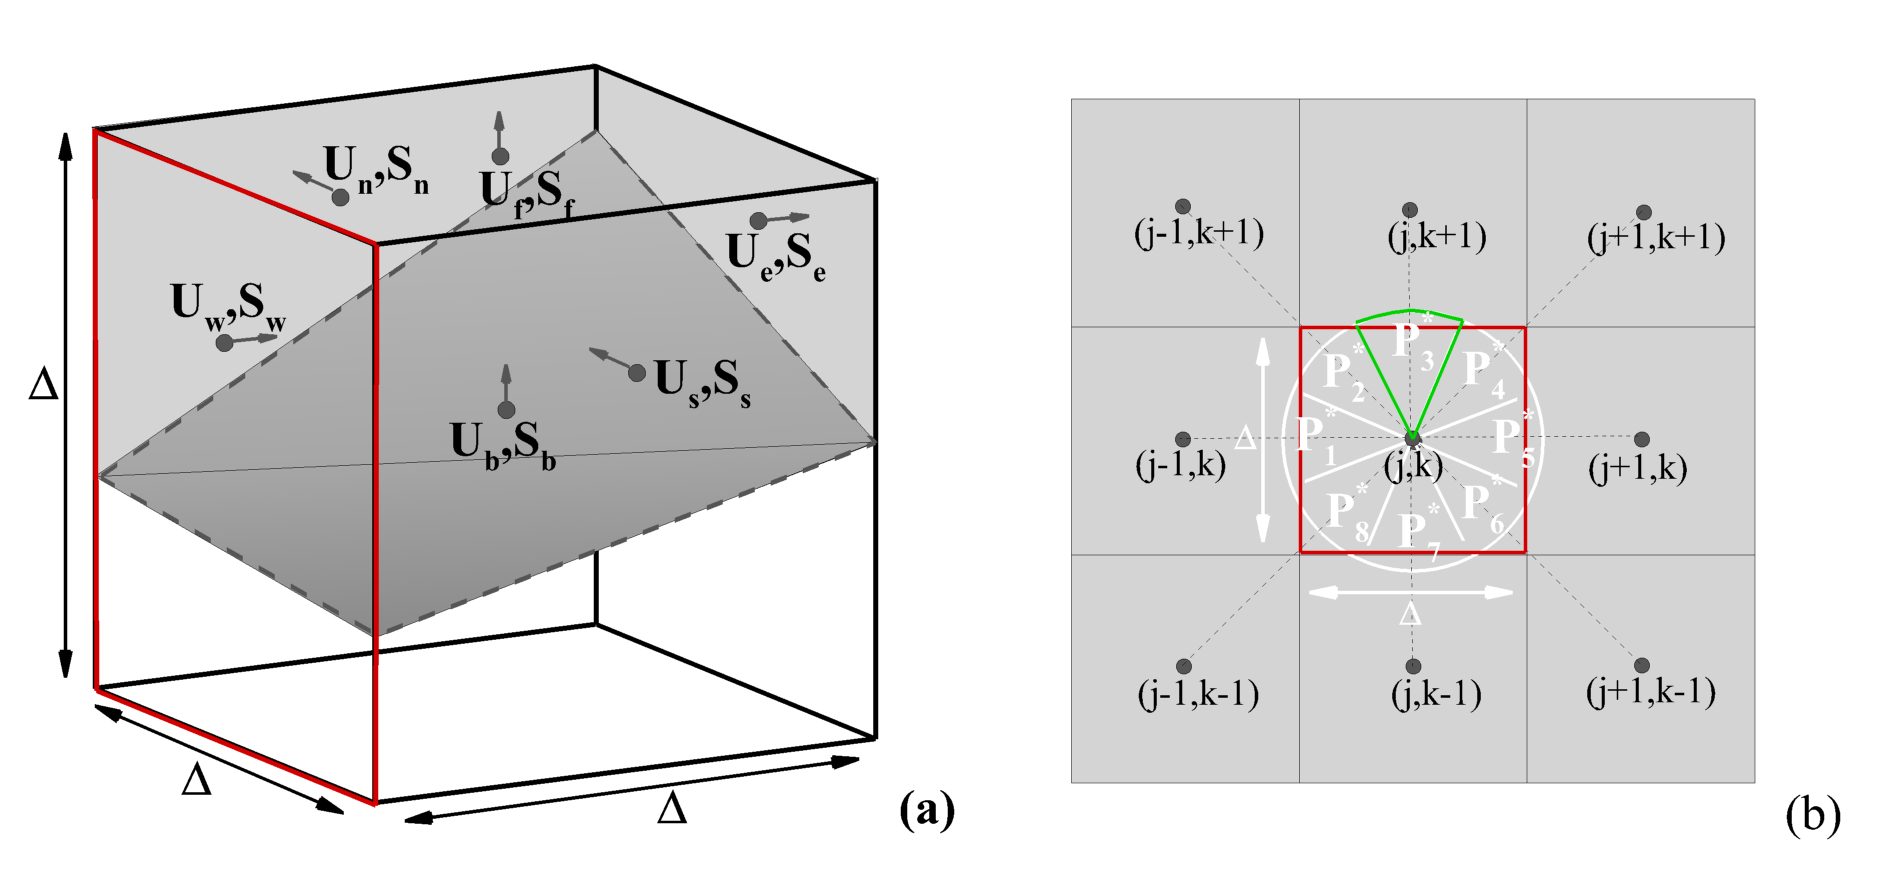
\includegraphics[width=16cm]{\EPSDIR/fig10_5.png} \\
	\vspace{-1mm} 
	\small \caption {{\it (a) Momentum fluxes balance for an arbitrary truncated cell of volume ${\mathcal V}$ where the $\overline{u_i}^*$ velocities ($U_i$ in the figure, $i=[e,w,n,s,b,f]$) are supported by the ${\mathcal S_i}$ surfaces in grey colour; the transparent volume is a part of the solid body. (b) Segmentation of the ${\mathcal S_w}$ arbitrary surface (red border) in eigth $P_p^*$ pieces of cake (the border of $P_3^*$ is indicated in green).}} 
\label{cheese0}
\end{center}
\end{figure}

The elliptic problem is re-written as a resolution of the linear system ${\mathcal P}.\Psi^{*}={\mathcal Q}$. In the standard Meso-NH version, $\nabla .\overline{\bf{u}}^{*}={\mathcal Q}$ is estimated using a finite difference approach. To uncouple the solid region from the fluid region, a null-divergence for pure solid cells is enforced and the balance of momentum fluxes is estimated by a finite volume approach for truncated cells (noted ${\mathcal Q}_{cct}$): 

\vspace{-0.25cm}
\begin{equation}
{\mathcal V} \nabla . \overline{\bf{u}}^{*} = \int_{\mathcal V_f} \nabla . \overline{\bf{u}}^{*} d{\mathcal V} + \int_{\mathcal V_s} \nabla \overline{\bf{u}}^{*} d{\mathcal V} = \sum \pm \overline{u_i}^{*}.{\mathcal S_i} = \sum \pm \widetilde{\Delta^2 \overline{u_i}^{*}}
\label{eqn_pres1}
\end{equation}
\vspace{-0.25cm}

where $\mathcal V= \Delta^3$ is the cell volume, $\mathcal V_f$ (resp. $\mathcal V_s$) the fluid (resp. solid) part of $\mathcal V$, ${\mathcal S_i}$ the cell surfaces where $i$ is the index of each surface orientation [e,w,n,s,b,f] as it illustrates in Figure~\ref{cheese0}-a. 

According to the Green-Ostrogradski theorem, the $\overline{u_i}^{*} {\mathcal S_i}$ calculation is the classical way of a CCT Cut-Cell Technique (Yang et al., 1997; Kim et al., 2001) to estimate the velocity divergence. A similar approach is here performed re-building the flux $\widetilde{\Delta^2 \overline{\bf{u}}^{*}}$ for truncated and solid cells.

\begin{figure}[!ht]
\begin{center}
   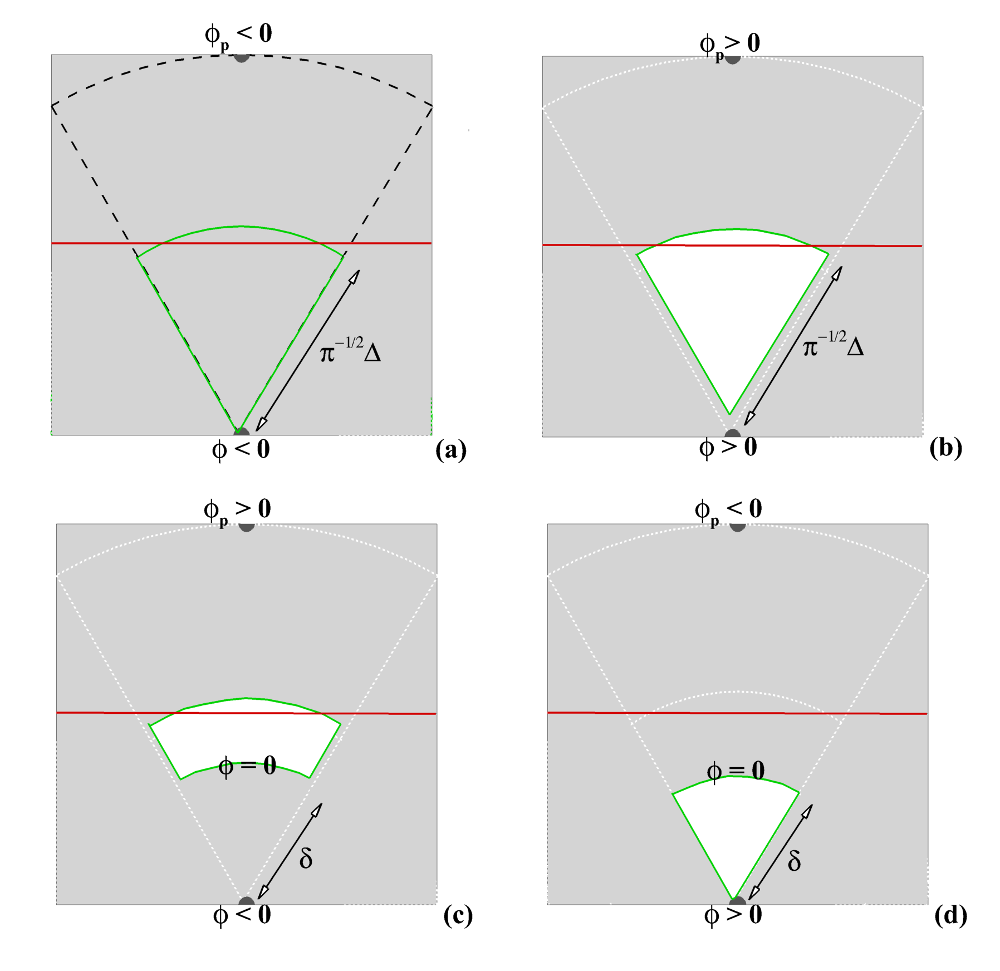
\includegraphics[width=16cm]{\EPSDIR/fig10_6.png} \\	
		\vspace{-1mm} 	
	\small \caption {{\it (a,b,c,d) $\pm \widetilde{\Delta^2 \overline{u_i}^{*}}$ calculations depending on the signs of $\phi_i=(\phi)$ and $\phi_p$ on an arbitrary piece of cake. The white (resp. grey) region corresponds to the solid (resp. fluid) one of $P_p^*$ (same colour code as in Fig.~\ref{cheese0}).}}
\label{cheese1}
\end{center}
\end{figure}

The $\pm \widetilde{\Delta^2 \overline{u_i}^{*}}$ calculation consists in a weighting of the out-fluxes and in-fluxes function of the fluid and cell surfaces ratio (Fig.~\ref{cheese0}-a). Figure~\ref{cheese0}-b gives an example of the west surface ($i=w$, red border) where $\widetilde{\Delta^2 \overline{u_w}^{*}}(j,k)$ is calculated using the LSF value $\phi=\phi_w$ and the ones of the eight adjacent nodes $\phi_p(j \pm 1,k \pm 1)$. A disk of radius $\sqrt[-1]{\pi}\Delta$ is split in eight 'piece of cake' segments $P_p^*$ ($p=[1:8]$). A LSF linear interpolation detects or not the interface location. In presence of an interface, its distance from the studied node is $0<\delta_p<\sqrt[-1]{\pi}\Delta$. Knowing $\delta_p$, the momentum fluxes balance is formulated for a non-moving body as $p$ is the index of the 'piece of cake' and $i$ the index of the cell surface:

\vspace{-0.25cm}
\begin{equation}
\widetilde{\Delta^2 \overline{u_i}^{*}} = \frac{\Delta^2}{8}[\overset{8}{\underset{p=1}{\sum}} {\mathcal H}(-\phi_p){\mathcal H}(-\phi_i)\overline{{\bf u_i}}^{*}
                    +\overset{8}{\underset{p=1}{\sum}} {\mathcal H}(-\phi_p\phi_i).|{\mathcal H}(-\phi_p)-\pi(\frac{\delta_p}{\Delta})^2|.
						 ({\mathcal H}(-\phi_p)\overline{{\bf u}}_p^{*}+{\mathcal H}(-\phi_i)\overline{{\bf u_i}}^{*})]
\label{eqn_pres3}						
\end{equation}
\vspace{-0.25cm}

The four encountered cases correspond to a pure fluid cell $\widetilde{\Delta^2 \overline{u_i}^{*}} = \frac{\Delta^2}{8}\overset{8}{\underset{p=1}{\sum}} \overline{{\bf u_i}}^{*}$ when $\phi_p<0$ and $\phi_i<0$ (Fig.~\ref{cheese1}-a); a pure solid cell $\widetilde{\Delta^2 \overline{u_i}^{*}} =0$ when $\phi_p>0$ and $\phi_i>0$ (Fig.~\ref{cheese1}-b); two types of truncated cells depending on the fluid/solid nature of the main node for which $\phi_p . \phi_i<0$ (Fig.~\ref{cheese1}-c/d). Using Equation~\eqref{eqn_pres3}, Equation~\eqref{eqn_pres1} is solved and leads to the RHS computation of the elliptic pressure equation. 

Knowing ${\mathcal Q}_{cct}$, the reflection concerns now the ${\mathcal P}$ matrix to invert. The classical interface condition on the potential $\Psi^{*}$ is a homogeneous Neumann condition $\frac{\partial \Psi^{*}}{\partial \phi}=0$. Using a Boundary Fitted Method (BFM), the interface condition of the moving or non-moving body (Auguste, 2010) appears only on the border of a numerical domain. Using an IBM and without any impact of this interface condition on the ${\mathcal P}$-coefficients, the impermeability character of solid obstacles is not achieved. Due to the inversion of the horizontal part of $\mathcal P$ by a Fast Fourier Transform (Schumann and Sweet, 1988), the solution of calculating ${\mathcal P}_{cct}$ appears to be problematic. The adopted solution consists in an iterative procedure as used in Meso-NH for non-flat problems. The non-respect of the $\Psi^*$-condition in ${\mathcal P}$ leads to a not well-posed system and the iterative procedure goes to spread to the entire fluid domain the enforcement of the null-divergence imposed on solid cells. The solution of the pseudo-Poisson equation brings to $\Psi^* \rightarrow \Psi^{*M}=\overset{M}{\underset{m=1}{\sum}}{\mathcal P}^{-1}.{\mathcal Q}_{cct}^{m}$ where $M$ is the number of iterations. This number is limited by a convergence criterion, which is a compromise between incompressibility satisfaction and CPU cost.
%
\section{Representation of subgrid turbulent exchange near the obstacles}
\label{S_WAL}
%
It is known that the $\frac{l_m}{l_\epsilon} \rightarrow 1$ is a reasonable approximation in non-homogeneous, non-isotropic turbulence such as in the near-wall region. This approximation is indeed retained in the present IBM implementation, which assumes $l_m=l_\epsilon$ (hereafter noted $l_m$ and called the mixing length). $l_m$ is equal to the numerical cut-off space scale sufficiently far from the ground bringing to a $\Delta \sqrt{e}$ turbulent viscosity. Near the ground and following the Prandtl idea consisting in the assumption of the linear variation of $l_m$ in the near-wall region, the upper limit of the mixing length is $min(kz,\Delta)$ ({\it k} is the von K\'arm\'an constant and $z$ is the altitude). 

\begin{figure}[!ht]
\begin{center}
   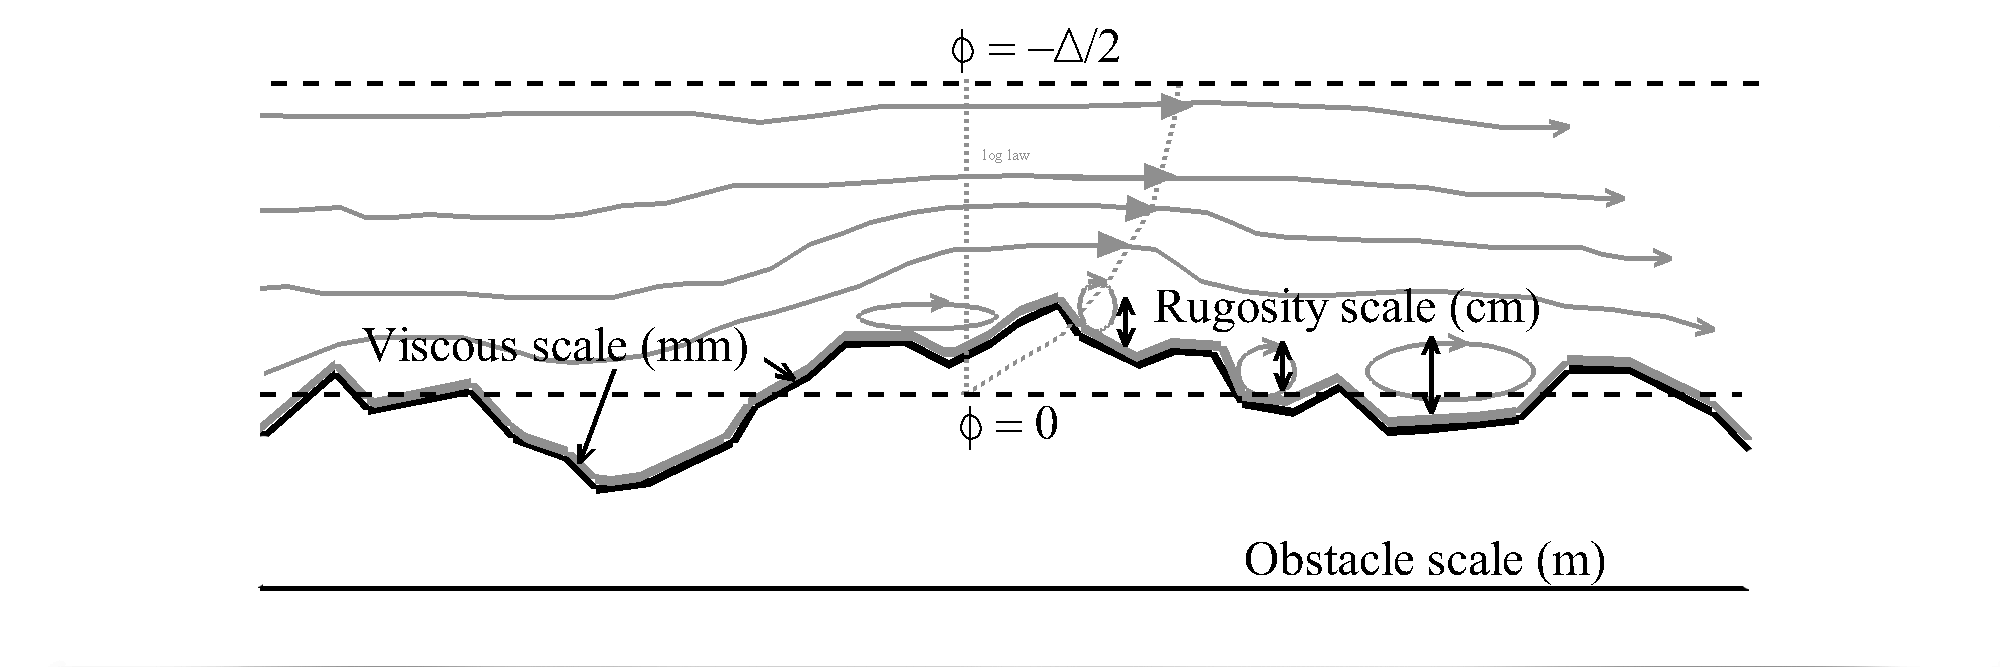
\includegraphics[width=16.cm]{\EPSDIR/fig10_7.png}	\\
   \vspace{-1mm} 
	\small \caption {{\it Illustration of the unresolved physical processes near a non-idealized solid wall (black line) in an atmospheric context: the length scale based on the viscous effects (grey line) is drastically smaller than the roughness length. The roughness length approaches the scale of smallest eddies and governs the log-law profile.}}
	\label{roughness}
\end{center}
\end{figure}

The turbulent characteristics are highly affected by a surface interaction. As a consequence and for LES, the subgrid turbulence scheme is modified in presence of immersed obstacles on the subgrid turbulent kinetic energy equation, mixing length computation and Reynolds stresses diagnosis.\\

{\bf The Subgrid Turbulent Kinetic Energy ($e$) condition}. The explicit-in-time resolution of the prognostic equation for subgrid turbulent kinetic energy claims a GCT forcing and an interface condition on $e$. Commonly, the $e$ profile is considered parabolical in the viscous sublayer (Bredberg, 2000; Craft et al., 2002) and constant in the inertial and wake/outer layers (Kalitzin et al., 2005; Capizzano, 2011). Due to the high turbulent Reynolds number $Re_t \approx {\mathcal O}(10^4-10^5)$ encountered, a homogeneous Neumann condition is applied at the immersed interface. The equilibrium between production and dissipation of $e$ could be discussed and controverted; this choice acts as a first stage in the IBM development.\\ 
 
{\bf The near-wall correction of the mixing length}. The von K\'arm\'an limitation due to immersed walls acts through the LSF and the upper limit on the mixing length $l_m$ near the interface becomes $min({\it k}z,-\phi, \Delta)$ with a banning of negative values in the solid region. Whatever the production of Subgrid Turbulent Kinetic Energy $e$, and the turbulent shear, the lower limit $l_m(-\phi \le 0)$ induces a null value of the diagnosed surface fluxes. In addition, a singularity appears in the dissipative term $\rho_r K_\epsilon e^{3/2}l_m^{-1}$. By a pragmatic reasoning, the singularity due to $l_m^{-1}(\phi \rightarrow 0^{-}) \rightarrow \infty$ amounts to say that modelled length scales are smaller than the Kolmogorov scale $(\nu^{3}\epsilon^{-1})^{\frac{1}{4}}$. Considering the Kolmogorov scale as modeled, the turbulence should vanish which is in contradiction with the dissipative term. In order to overcome this ill-posed problem, a lower limit has to be specified for $l_m$. In the study of atmospheric flows around buildings, a characteristic thickness of the viscous layer $H/\sqrt{Re}$ can be defined around a $H$ bluff body for a Reynolds number based on the obstacle scale: $H \approx {\mathcal O}(10m); Re \approx {\mathcal O}(10^7)$. This thickness estimate is also proportional to $E\nu/u^*$ ($E \approx 9.8$ is commonly employed) where the friction velocity $u^*$ is about the centimeter per second. Following these estimates, the length scale due to the viscous effects $z_\nu^{ib}$ belongs to the millimetres domain in the expected atmospheric cases. Looking after a building surface and its large heterogeneity (door, windows, surface characteristics), its roughness length $z_0^{ib}$ is at least in the decimeter domain and $z_0^{ib} > z_\nu^{ib}$ (Illustration in Fig.~\ref{roughness}). For low $Re$ and smooth surfaces, $z_\nu^{ib}>z_0^{ib}$ could be encountered. Therefore, we assume $z^{ib}=max(z_0^{ib},z_\nu^{ib})$ and that $z^{ib}$ is related to the size of smallest unresolved eddies near walls (i.e. dissipative scale). The mixing length near wall is $z^{ib}<l_m<min({\it k}z,-\phi,\Delta)$. \\

{\bf The turbulent fluxes correction}. The $\overline{\psi}$-gradient and the turbulent diffusion $\mathcal{O}(z^{ib}\sqrt{e})$ prescribe the turbulent fluxes at the immersed interfaces. As a first step in the Meso-NH-IBM implementation, no-flux condition on the mean potential temperature is imposed such that the sensible heat flux is zero. Writing the mean velocity field at $B$ such as $\overline{{\bf u}}=\overline{u_t}{\bf t}$, $\overline{u_t}(B)$ is needed to recover a gradient consistent with the turbulent shear. Considering the Prandtl (1925) or K\'arm\'an (1930) theories, the logarithmic profile is assumed in the vicinity of the wall according to $\overline{u}_t(z)  = \frac{u^*}{{\it k}} ln (1+\frac{z}{z^{ib}})$. Considering $\Delta$ as the limit of the resolved scales, most of the turbulent kinetic energy $\frac{1}{2}(\overline{u'^2}+\overline{v'^2}+\overline{w'^2})$ is contained in the subgrid one when $-\phi<\Delta$ and such as $K_{tke}\sqrt{e}$ with a constant $K_{tke} \gtrsim 1$. This assumption is reinforced by the homogeneous Neumann condition applied on $e$. This approach derives from the RANS (Reynolds-Averaged Navier Stokes) approaches and the velocity friction is formulated as $u^*=K_{tke}\sqrt[4]{C_\mu}\sqrt{e}$ where $C_\mu$ is a constant evolving between 0.03 (atmospheric applications) and 0.09 (fluid mechanics applications). Adding a damping function for the viscous cases (low turbulent Reynolds number, $Re_t<20$), the tangent wall velocity at the interface is written such as: 

\vspace{-0.25cm}
\begin{equation}
\overline{u}_t(B) = \frac{K_{tke}\sqrt[4]{C_\mu}\sqrt{e(\phi=-\Delta/2)}}{\it k}ln \left(1+\frac{\Delta}{z^{ib}} \left [1-e^{-20z^{ib}\Delta^{-1}} \right] \right)
\label{eqn_les}
\end{equation} 
\vspace{-0.25cm}

Finally the pragmatic limitation $\overline{u}_t(B) \le \overline{u_t}(\phi=-\Delta /2)$ operates if the $e$ value is too high. The proposed dynamic wall-model evolves between the no-slip and free-slip conditions. If the subgrid turbulence is weak or if the physical problem is fully resolved, the viscous layer is well-modelled and $\overline{u_t}(B) \rightarrow 0$. Otherwise for an intense subgrid turbulence or a fully unresolved problem, the shear due to the wall presence is not perceived and $\frac{d \overline{u_t}}{d n}\big|_{B} \rightarrow 0$. The wall-model establishes an equilibrium between the production of $e$ and the mean parietal friction. Note that the use of a log-law model near a singularity such as sharp edges and corners could be called into question. After numerical investigations for a single cube, $K_{tke} \sqrt[4]{C_\mu} \approx 1$ appears as a suitable choice. 
%
\section{References}
%
\decrefname
Auguste, F., 2010:
Instabilités de sillage et de trajectoire dans un fluide visqueux.
{\it PhD thesis, University of Toulouse}, 313 p.
\decrefname
Auguste, F., G. R\'ea, R. Paoli, C. Lac, V. Masson, and D. Cariolle, 2019:
Implementation of an immersed boundary method in the Meso-NH v5.2 model: applications to an idealized urban environment.
{\it Geoscientific Model Development}, {\bf 12(6)}, 2607-2633.
\decrefname
Aumond, P., V. Masson, C. Lac, B. Gauvreau, S. Dupont, and M. Berengier, 2013:
Including the drag effects of canopies: real case large-eddy simulation studies.
{\it Bound.-lay. Met.}, {\bf 146}, 65-80.
\decrefname
Bredberg, J., 2000:
On the wall boundary condition for turbulence models.
{\it Chalmers University of Technology, Department of Thermo and Fluid Dynamics. Goteborg.}, {\bf Internal Report 00/4}, 21 p.
\decrefname
Capizzano, F., 2011:
Turbulent wall model for immersed boundary methods.
{\it AIAA journal}, {\bf 49(11)}, 2367-2381.
\decrefname
Clarke, D. K., M. D. Salas, and H. A. Hassan, 1986:
Euler calculations for multielement airfoils using Cartesian grids.
{\it AIAA journal}, {\bf 24(3)}, 353-358.
\decrefname
Craft, T., S. Gant, A. Gerasimov, H. Iacovides, and B. Launder, 2002:
Wall Functions Strategies for Use in Turbulent Flow CFD. 
{\it J. Heat transfer}, {\bf 1}, 3-14.
\decrefname
Franke, R., 1982:
Scattered data interpolation, tests of some methods.
{\it Math. Comput.}, {\bf 38(157)}, 181-200.
\decrefname
Goldstein, D., R. Handler, and L. Sirovich, 1993:
Modeling a no-slip flow boundary with an external force field.
{\it J. Comput. Phys.}, {\bf 105(2)}, 354-366.
\decrefname
Kalitzin, G., G. Medic, G. Iaccarino, and P. Durbin, 2005:
Near-wall behavior of RANS turbulence models and implications for wall functions.
{\it J. Comput. Phys.}, {\bf 204(1)}, 265-291.
\decrefname
Kármán, T. von, 1930:
Mechanische \"Anlichkeit und Turbulenz.
{\it Nachrichten von der Gesellschaft der Wissenschaften zu Göttingen, Mathematisch-Physikalische Klasse}, 58-76.
\decrefname
Kempe, T., and J. Fröhlich, 2012: 
An improved immersed boundary method with direct forcing for the simulation of particle laden flows.
{\it J. Comput. Phys.}, {\bf 231(9)}, 3663-3684.
\decrefname
Kim, J., D. Kim, and H. Choi, 2001: 
An immersed-boundary finite-volume method for simulations of flow in complex geometries.
{\it J. Comput. Phys.}, {\bf 171(1)}, 132-150.
\decrefname
Leveque, R. J., and Z. Li, 1994:
The immersed interface method for elliptic equations with discontinuous coefficients and singular sources.
{\it SIAM Journal on Numerical Analysis}, {\bf 31(4)}, 1019-1044.
\decrefname
Lundquist, K. A., F. K. Chow, and J. K. Lundquist, 2010:
An immersed boundary method for the Weather Research and Forecasting model.
{\it Mon. Wea. Rev.}, {\bf 138(3)}, 796-817.
\decrefname
Lundquist, K. A., F. K. Chow, and J. K. Lundquist, 2012:
An immersed boundary method enabling large-eddy simulations of flow over complex terrain in the WRF model.
{\it Mon. Wea. Rev.}, {\bf 140(12)}, 3936-3955.
\decrefname
Mittal, R., and G. Iaccarino, 2005:
Immersed Boundary Methods.
{\it Annu. Rev. Fluid Mech.}, {\bf 37}, 239-261.
\decrefname
Mohd-Yusof, J., 1997:
Combined immersed-boundary/B-spline method for simulations of flow in complex geometries.
{\it Center for Turbulence Research Annual Research Briefs}, 317-327.
\decrefname
Peskin, C. S., 1972:
Flow patterns around heart valves: a numerical method.
{\it J. Comput. Phys.}, {\bf 10(2)}, 252-271.
\decrefname
Pierson, J.-L., 2015:
Traversée d’une interface entre deux fluides par une sphère.
{\it PhD thesis, University of Toulouse}, 226 p.
\decrefname
Prandtl, L., 1925:
Bericht über Untersuchungen zur ausgebildeten Turbulenz.
{\it Z. Angew. Math., Meth.}, {\bf 5}, 136-139.
\decrefname
Schumann, U., and R. Sweet, 1988:
Fast Fourier Transforms for direct solution of Poisson's equations with staggered boundary conditions.
{\it J. Comput. Phys.}, {\bf 75}, 123-137.
\decrefname
Sussman, M., P. Smereka, and S. Osher, 1994:
A level set approach for computing solutions to incompressible two-phase flow.
{\it J. Comput. Phys.}, {\bf 114(1)}, 146-159.
\decrefname
Tseng, Y. H., and J. H. Ferziger, 2003:
A ghost-cell immersed boundary method for flow in complex geometry.
{\it J. Comput. Phys.}, {\bf 192(2)}, 593-623.
\decrefname
Yang, G., D. M. Causon, D. M. Ingram, R. Saunders, and P. Batten, 1997:
A Cartesian cut cell method for compressible flows part A: Static body problems.
{\it Aeronaut. J.}, {\bf 101(1002)}, 47-56.
\decrefname
Ye, T., R. Mittal, H. S. Udaykumar, and W. Shyy, 1999:
An accurate Cartesian grid method for viscous incompressible flows with complex immersed boundaries.
{\it J. Comput. Phys.}, {\bf 156(2)}, 209-240.
